%##################################################
% FoF
%##################################################
\section{Friends-of-Friends algorithm}
\bartchapterimage{heic1006a_small.jpg}
\bartthumb{thumbs/heic1006a.png}

\subsection{Description}
\begin{frame}
    \frametitle{Friends-of-Friends algorithm}
    \begin{columns}
        \begin{column}{0.5\textwidth}
            \begin{minipage}[c][0.4\textheight][c]{\linewidth}
                \begin{tikzpicture}[scale=0.4]
                    \tikzstyle{dots}=[
                        draw,
                        shape=circle,
                        fill=black,
                        text=white,
                        scale=0.5,
                    ]
                    \tikzstyle{searched}=[line width=1.5pt, blue!90!white]
                    \tikzstyle{linked}=[line width=2pt]
                    \node[dots] (1) at (0, 1) {1};
                    \node[dots] (2) at (1, 2) {2};
                    \node[dots] (3) at (3, 4) {3};
                    \node[dots] (4) at (4, 7) {4};
                    \node[dots] (5) at (3, 6) {5};
                    \node[dots] (6) at (8, 4) {6};
                    \node[dots] (7) at (7, 3) {7};
                    \node[dots] (8) at (10, 1) {8};

                    \draw[searched, visible on=<2>] (1) circle (3);
                    \draw[blue, line width=1pt, visible on=<2>]
                        (1.center) -- ($ (1.center) + (3, 0) $)
                        node[below] at ($ (1.center) + (1.5, 0) $) {$b$};

                    \draw[linked, green, visible on=<3->] (1) -- (2);
                    \node[dots, fill=green, text=black, visible on=<3->] (1)
                        at (0, 1) {1};
                    \node[dots, fill=green, text=black, visible on=<3->] (2)
                        at (1, 2) {2};

                    \draw[searched, visible on=<4>] (2) circle (3);

                    \draw[linked, green, visible on=<5->] (2) -- (3);
                    \node[dots, fill=green, text=black, visible on=<5->] (3)
                        at (3, 4) {3};

                    \draw[searched, visible on=<6>] (3) circle (3);

                    \draw[linked, green, visible on=<7->] (3) -- (5);
                    \node[dots, fill=green, text=black, visible on=<7->] (5)
                        at (3, 6) {5};

                    \draw[searched, visible on=<8>] (5) circle (3);

                    \draw[linked, green, visible on=<9->] (4) -- (5);
                    \node[dots, fill=green, text=black, visible on=<9->] (4)
                        at (4, 7) {4};

                    \draw[searched, visible on=<10>] (6) circle (3);

                    \draw[linked, purple, visible on=<10->] (6) -- (7);
                    \node[dots, fill=purple, text=black, visible on=<10->] (6)
                        at (8, 4) {6};
                    \node[dots, fill=purple, text=black, visible on=<10->] (7)
                        at (7, 3) {7};

                    \draw[searched, visible on=<11>] (7) circle (3);

                    \node[dots, fill=orange, text=black, visible on=<12>] (8)
                        at (10, 1) {8};
                \end{tikzpicture}
            \end{minipage}
        \end{column}
        \begin{column}{0.5\textwidth}
            \begin{minipage}[c][0.4\textheight][c]{\linewidth}
                \begin{block}{}
                    \begin{enumerate}
                        \item<2-> Two galaxies linked if their separation is
                            less than the linking length $b$
                        \item<3-> Loop over each galaxies to find galaxies
                            linked together through another one
                        \item<12-> Finally, space partitioned into galaxy
                            groups
                    \end{enumerate}
                \end{block}
            \end{minipage}
        \end{column}
    \end{columns}
\end{frame}

\begin{frame}
    \frametitle{Friends-of-Friends algorithm}

    \begin{columns}
        \begin{column}{0.5\textwidth}
            \begin{block}{Linking lengths}
                \begin{enumerate}
                    \item<1-> Characterization of the density:
                        $\cfrac{\delta n}{n}=\cfrac{3}{4\pi b^3}-1$
                    \item<2-> Redshift distortions implies to split linking
                        length in two classes:
                        \begin{itemize}
                            \item transverse $b_\bot$
                            \item parallel (line-of-sight) $b_\parallel$
                        \end{itemize}
                    \item<3-> Optimization of linking lengths with tests
                \end{enumerate}
            \end{block}
        \end{column}
        \begin{column}{0.5\textwidth}
            \begin{adjustbox}{max width=\linewidth}
                \begin{tabular}{llllcrl}
                    \toprule%
                    \toprule%
                    Authors & sample & \multicolumn{1}{c}{$b_\perp$} &
                        \multicolumn{1}{c}{$b_\parallel$} &
                    \multicolumn{1}{c}{$b_\parallel/b_\perp$} & $\delta n/n$ \\
                    \toprule%
                    Huchra \& Geller 82     & CfA     & 0.23  & 1.34
                        & \ \ \ \ 6.3 & 20\\
                    Ramella et al. 89       & CfA2    & 0.14  & 1.9   & 13
                        & 80\\
                    Trasarti-Battistoni 98  & PPS2    & 0.13  & 1.7   & 13
                        & 108\\
                    Merchan \& Zand'z 02    & 2dFGRS  & 0.14  & 1.4   & 10
                        & 80\\
                    Eke et al. 04           & 2dFGRS  & 0.13  & 1.43  & 11
                        & 178\\
                    Berlind et al. 06       & SDSS    & 0.14  & 0.75
                        & \ \ \ \ 5.4 & 86\\
                    Tago et al. 10          & SDSS    & 0.075  & 0.75  & 10
                        & 565 \\
                    Robotham et al. 11      & GAMA    & 0.060  & 1.08  & 18
                        & 1100\\
                    Tempel et al. 14 ($M_r$$<$$-19$)        & SDSS    & 0.11
                        & 1.1 & 10 & 178 \\
                    Tempel et al. 14 ($M_r$$<$$-21$)        & SDSS    & 0.066
                        & 0.67 & 10 & 830 \\
                    \bottomrule%
                \end{tabular}
            \end{adjustbox}
        \end{column}
    \end{columns}
\end{frame}

\subsection{Analysis}
\begin{frame}
    \frametitle{Friends-of-Friends algorithm}

    \begin{columns}
        \begin{column}{0.4\textwidth}
            \begin{minipage}[c][0.7\textheight][c]{\linewidth}
                \begin{block}{Tests}
                    \begin{itemize}
                        \item<3-> Completeness
                        \item<5-> Reliability
                        \item<6-> Fragmentation
                        \item<7-> Merging
                    \end{itemize}
                \end{block}
            \end{minipage}
        \end{column}
        \begin{column}{0.6\textwidth}
            \begin{minipage}[c][0.7\textheight][c]{\linewidth}
                \begin{tikzpicture}[scale=0.25]
                    \tikzstyle{dots}=[
                        draw,
                        shape=circle,
                        fill=black,
                        text=white,
                        scale=0.5,
                    ]
                    \tikzstyle{dots2}=[
                        draw,
                        shape=circle,
                        fill=black,
                        text=white,
                        scale=0.5,
                        shift={(8, 0)},
                    ]
                    \tikzstyle{TG}=[line width=1.5pt, green!60!black]
                    \tikzstyle{EG}=[line width=1.5pt, red!60!black]
                    \tikzstyle{links}=[->, line width=2pt]

                    \draw[fill, green!60!black, opacity=0.3]
                        (0, -3) rectangle (13.5, 10);
                    \node[green!60!black, below]
                        at (6.75, -3) {Real space};
                    \draw[fill, red!60!black, opacity=0.3]
                        (13.5, -3) rectangle (28, 10);
                    \node[red!60!black, below]
                        at (20.25, -3) {Redshift space};

                    \node[dots] (1) at (4, 1) {};
                    \node[dots] (2) at (3, 2) {};
                    \node[dots] (3) at (4, 4) {};
                    \node[dots] (4) at (4, 7) {};
                    \node[dots] (5) at (3, 6) {};
                    \node[dots] (6) at (8, 4) {};
                    \node[dots] (7) at (6, 3) {};
                    \node[dots] (8) at (8, 1) {};
                    \node[dots] (9) at (9, 3) {};

                    \node[dots2] (1E) at (1) {};
                    \node[dots2] (2E) at (2) {};
                    \node[dots2] (3E) at (3) {};
                    \node[dots2] (4E) at (4) {};
                    \node[dots2] (5E) at (5) {};
                    \node[dots2] (6E) at (6) {};
                    \node[dots2] (7E) at (7) {};
                    \node[dots2] (8E) at (8) {};
                    \node[dots2] (9E) at (9) {};

                    \draw[TG] ([shift={(0, 1)}]7) circle (4.5);
                    \draw[EG, visible on=<1-5>] (3E) circle (4);

                    \draw[links, orange, visible on=<2>] (3E) -- (3);

                    \draw[EG, dashed, visible on=<3-4>] (3) circle (4);

                    \draw[TG, dashed, visible on=<5>]
                        ([shift={(0, 1)}]7E) circle (4.5);

                    \draw[EG, visible on=<6>] (3E) circle (3);
                    \draw[EG, dashed, visible on=<6>] (9E) circle (2);
                    \draw[links, orange, visible on=<6>] (3E) -- (3);
                    \draw[links, orange, dashed, visible on=<6>] (9E) -- (9);

                    \node[dots, visible on=<7>] (10) at (3, -1) {};
                    \node[dots, visible on=<7>] (11) at (4, -2) {};
                    \node[dots, visible on=<7>] (12) at (2, -2) {};
                    \node[dots, visible on=<7>] (13) at (3, 0) {};
                    \node[dots2, visible on=<7>] (10E) at (10) {};
                    \node[dots2, visible on=<7>] (11E) at (11) {};
                    \node[dots2, visible on=<7>] (12E) at (12) {};
                    \node[dots2, visible on=<7>] (13E) at (13) {};
                    \draw[TG, dashed, visible on=<7>] (10) circle (1.5);
                    \draw[EG, dashed, visible on=<7>] (7E) circle (6);
                    \draw[links, orange, dashed, visible on=<7>] (10) -- (10E);
                    \draw[links, orange, visible on=<7>] (3) -- (3E);
                \end{tikzpicture}
            \end{minipage}
        \end{column}
    \end{columns}
\end{frame}

\begin{frame}
    \frametitle{Friends-of-Friends algorithm}
    \begin{block}{Optimization}
        \begin{itemize}
            \item<1-> $16\times16$ grid of linking lengths
            \item<2-> Compute our statistics for each set of parameters
            \item<3-> Optimal linking lengths not obvious
        \end{itemize}
    \end{block}
\end{frame}

% \begin{frame}
    % \begin{minipage}{\linewidth}
        % \centering
        % 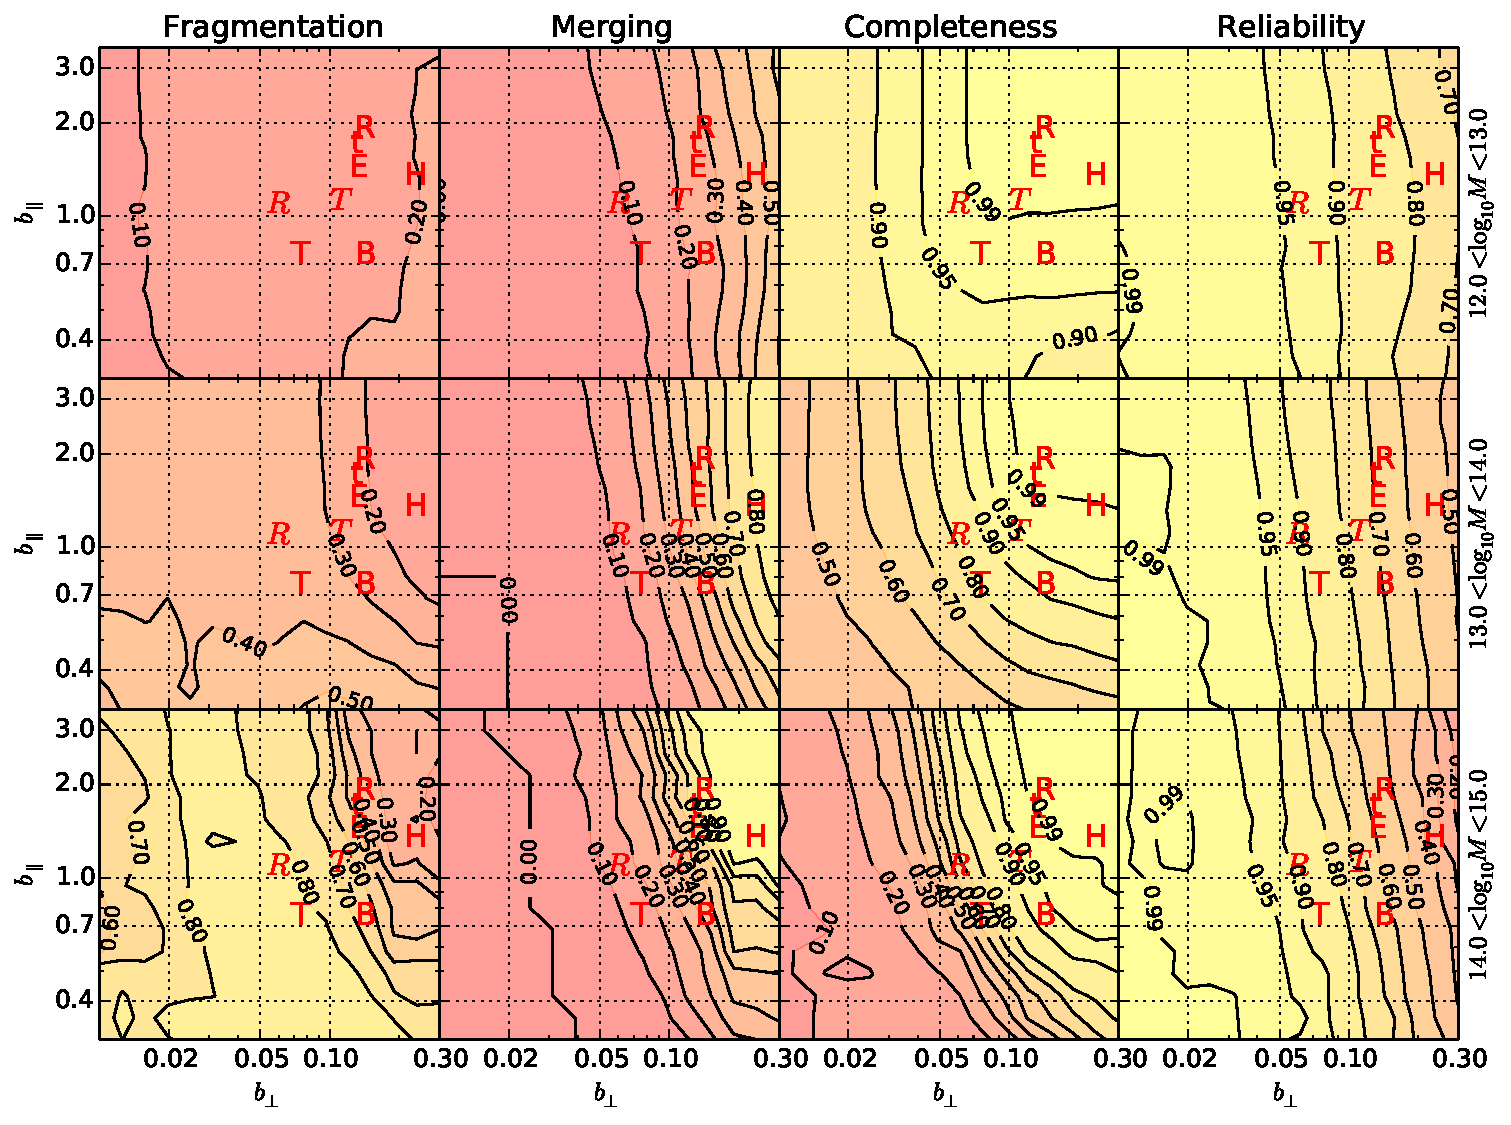
\includegraphics[height=0.8\textheight]{FMCR.pdf}
    % \end{minipage}
% \end{frame}

\begin{frame}
    \begin{columns}
        \begin{column}{0.55\textwidth}
            \begin{block}{Quality factors}
                \begin{enumerate}
                    \item<1-> Local quality: \\$Q_\mathrm{local}=\sqrt{%
                            {\left(1-C\right)}^2 + {\left(1-R\right)}^2
                        }$
                    \item<2-> Global quality: \\$Q_\mathrm{global}=\sqrt{%
                            F^2 + M^2
                        }$
                \end{enumerate}
            \end{block}
        \end{column}
        \begin{column}{0.45\textwidth}
            \centering
            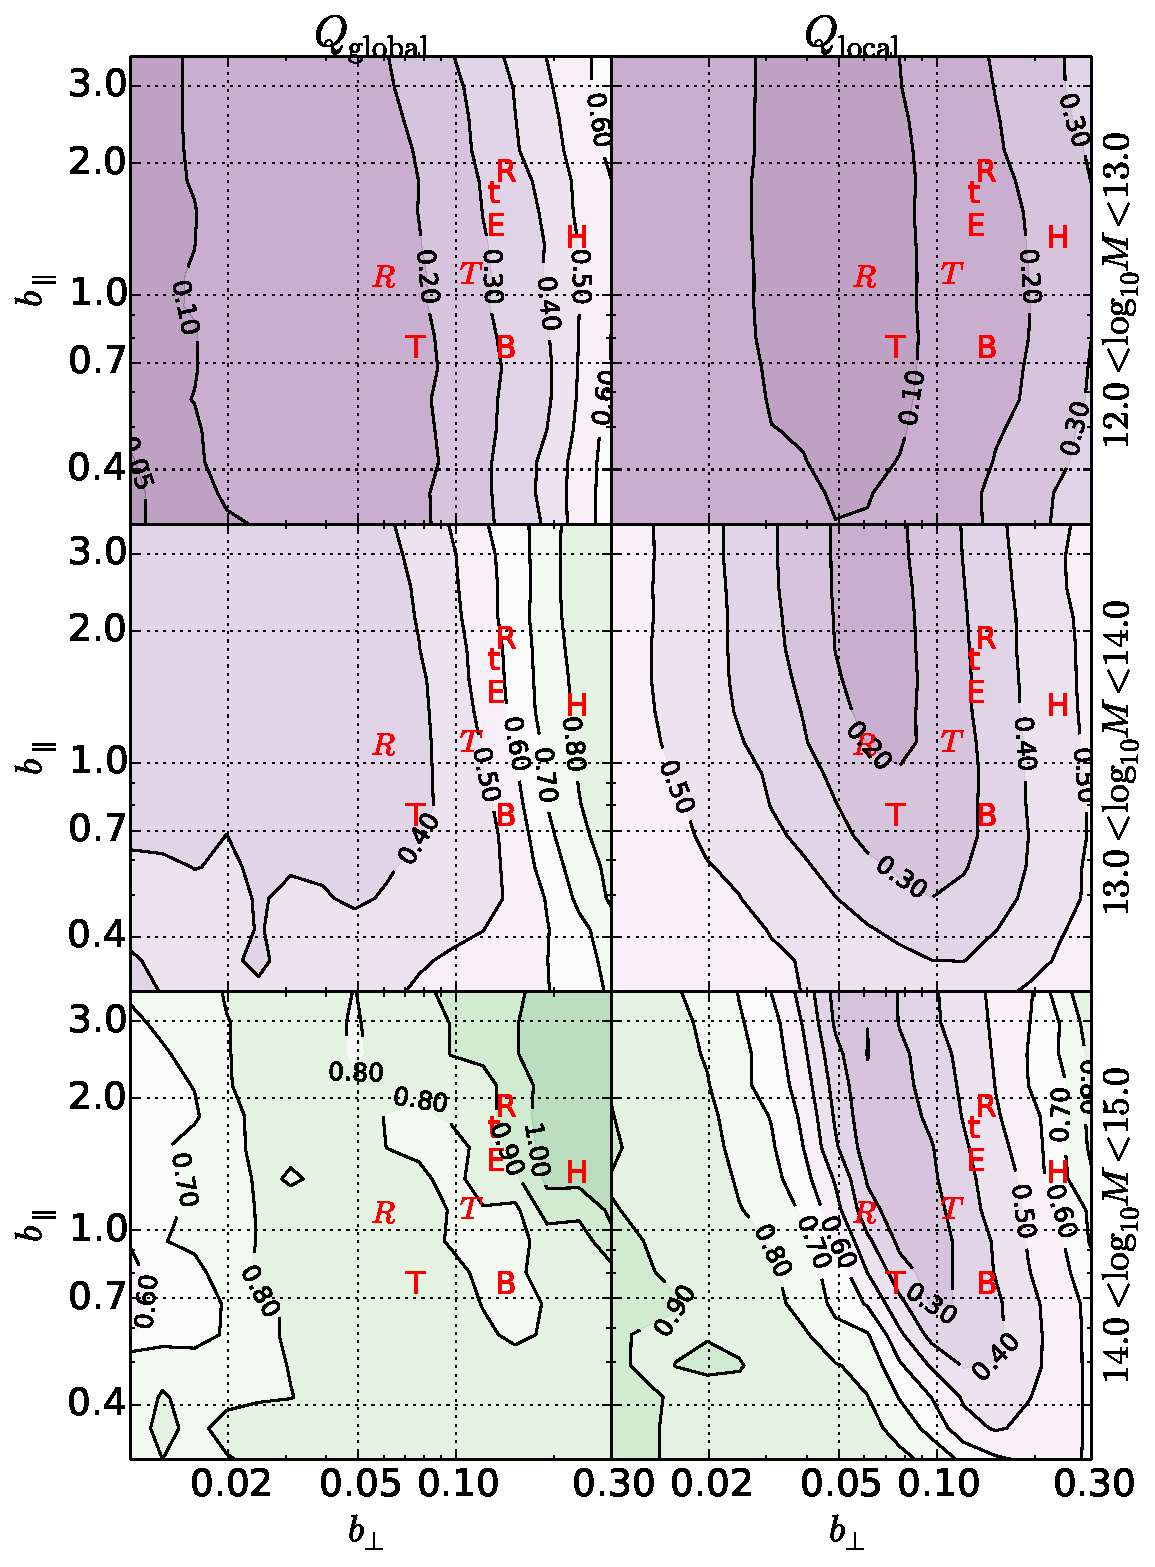
\includegraphics[height=0.75\textheight]{quality.pdf}
        \end{column}
    \end{columns}
\end{frame}

\subsection{Conclusions}

\begin{frame}
    \frametitle{Friends-of-Friends}
    \begin{block}{Conclusions}
        \begin{itemize}
            \item<1-> FoF optimized to $b_\bot=0.07$ and $b_\parallel=1.1$
            \item<2-> Optimization depends on scientific goal
            \item<3-> Contamination by interlopers is inevitable
            \item<4-> Fragmentation for high mass galaxy groups important
        \end{itemize}
    \end{block}
\end{frame}

% vim: set tw=79:
